\subsection{UCB versus $\epsilon$-greedy for $k$-bandit problem}

\paragraph{1.}
We randomly generated to means using a uniform random distribution,
where for each experiment the means where generated again.
To get the Lai-Robbins lower bound, we reuse the formulation of the KL-Divergence from task
5.4.3 . In the following plots, the experimental $l(t)$ curves can be seen together with the 
theoretical lower bound found by Lai-Robbins.
\begin{figure}[ht]
    \centering
    \begin{subfigure}{0.45}
        \centering
        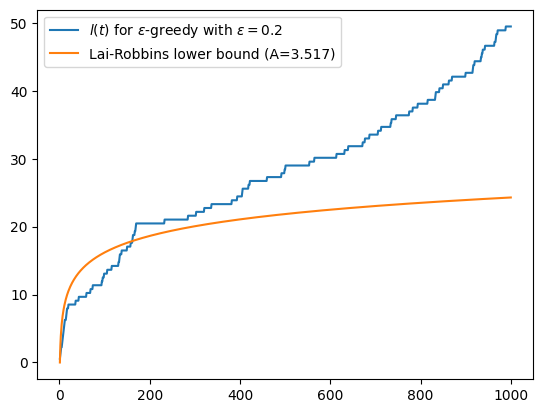
\includegraphics[scale=0.5]{figures/e02.png}
    \end{subfigure}  
    \begin{subfigure}{0.45}
        \centering
        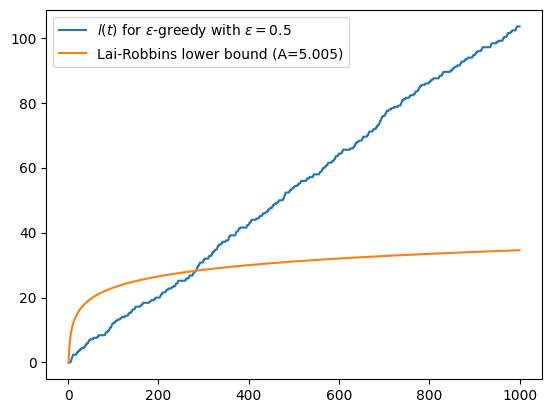
\includegraphics[scale=0.5]{figures/e05.png}
    \end{subfigure} 
    \begin{subfigure}{0.45}
        \centering
        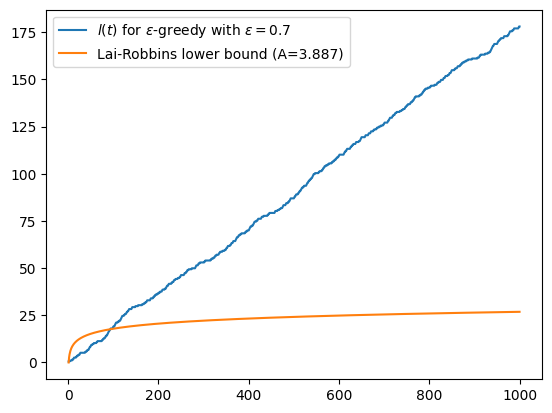
\includegraphics[scale=0.5]{figures/e07.png}
    \end{subfigure} 
    \begin{subfigure}{0.45}
        \centering
        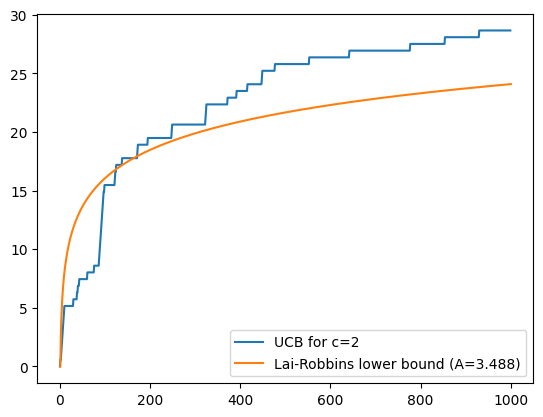
\includegraphics[scale=0.5]{figures/ucb.png}
    \end{subfigure}   
\end{figure}

\paragraph{2.}
Below we listed our observed correct decisions for the different strategies
\begin{itemize}
    \item UCB method: Correct: 0.7232\%
    \item $\epsilon$-greedy ($\epsilon=$): Correct: \%
    \item $\epsilon$-greedy ($\epsilon=$): Correct: \%
    \item $\epsilon$-greedy ($\epsilon=$): Correct: \%
\end{itemize}
If the c is smaller, the strategy explores less since the optimistic bounds
get smaller.
%python output
%For the UCB method, the following 
%Correct: 0.7232008424621057
%a1=0.7232008424621057, delta a1=0.0
%a2=0.14979742584010658, delta a2=0.5734034166219991
%q*: 0.7232008424621057
%mean regret: 0.028670170831099955